\documentclass[11pt,twoside,openright]{book}
\usepackage{bayesinstitute}
\renewcommand{\BookNumber}{1}
\renewcommand{\BookTitle}{The Opportunity}
\renewcommand{\BookSubtitle}{How to Find a Market Worth Serving and a Business Worth Building}
\renewcommand{\BookTagline}{How to Find a Market Worth Serving\\and a Business Worth Building}
\renewcommand{\BookQuestion}{Is there a game worth playing, and can I see the opening?}
\renewcommand{\BookScope}{This book develops the judgment needed to choose a business: the founder's starting position, ambition, decisions under uncertainty, markets, customers, positioning, and evidence of demand.}
\newcommand{\BookCoverTitle}{Opportunity}

\renewcommand{\BookTitle}{The Reading Specimen}
\renewcommand{\BookSubtitle}{An editorial and data-design specimen}
\renewcommand{\BookTagline}{A specimen for sustained reading\\and practical business lessons.}
\renewcommand{\BookQuestion}{How should an idea become a useful business decision?}
\renewcommand{\BookScope}{This specimen demonstrates the proposed print system with prose excerpts from the existing manuscript. Its examples of delivery economics are illustrative, not forecasts.}
\begin{document}
\BIFrontMatter
\chapter{Choosing the game}
\ChapterLead{The economics of entrepreneurship and wealth creation.}
\section{The wager}
Imagine two people who are equally capable at twenty-eight. Both are engineers. Both are unusually curious, willing to work hard, and capable of learning things that most people find difficult. One accepts a job at a good company. The other starts a company.

Ten years later, the first might have a distinguished career, a substantial investment portfolio, a home, and the ability to leave a job without financial panic. The second might have a company valued at a hundred million dollars. Or a company that brings in enough cash to employ twelve people and pay its founder handsomely. Or an exhausted bank account and an excellent education in the things that go wrong.

If you want to understand entrepreneurship, you must resist the temptation to compare the employee in the first story with the unusually successful founder in the second. The economically relevant comparison is between \emph{the choices as they appeared at twenty-eight}, before anyone knew which outcome would occur.

In retrospect, successful companies look almost destined to exist. We explain their triumph with a neat sequence: the founder saw a problem, built something brilliant, found a market, hired exceptional people, and persevered. But at the beginning the founder was surrounded by alternative explanations for everything. Maybe the problem was not important. Maybe customers would not pay. Maybe a competitor would arrive first. Maybe the technology would change. Maybe the founder would lose interest. Maybe another path would have been better.

Entrepreneurship begins with choosing to act amid these competing possibilities. That is what makes it both exciting and hazardous.

People often say they want to start a company because they want to become rich. We should not pretend that this is a shameful or trivial reason. Wealth can buy time, independence, protection from emergencies, the ability to support people one loves, and freedom to pursue difficult work without asking for permission. A sufficiently successful business can also create opportunities for other people on a scale that personal savings cannot.

But “I want to be rich” is not yet a theory of entrepreneurship. It does not tell us whether founding a company is the best way to reach that goal. It does not tell us what kind of company to build, what risks to take, or how to know whether the effort is working. Indeed, it does not even tell us what \emph{rich} means.

A person earning a large salary and saving consistently may become wealthy. A person who builds a profitable company and owns nearly all of it may become wealthy. A person who creates a fast-growing company may end up holding valuable shares that cannot easily be sold. A person who raises substantial venture capital may control a famous business while owning a comparatively small part of it. Someone else may sell a modest company and obtain more spendable wealth than the founder of a celebrated unicorn.

The first useful distinction, therefore, is between \textbf{income, wealth, control, and freedom}. They often travel together, but they are not the same thing.

\begin{KeyIdea}
The economically relevant comparison is between the choices as they appeared
before anyone knew which outcome would occur.
\end{KeyIdea}
\NotesSection
This specimen draws on the opening of the existing Chapter 1 manuscript,
``Why Play the Game?'' The production chapter will carry its own research notes.
\chapter{Keeping the promise}
\ChapterLead{A product is a promise plus an operating system for keeping it.}
\begin{LessonBrief}
\BriefPoint{The question}{What must happen for the customer to receive the promised result?}
\BriefPoint{The insight}{The offering includes the work, handoffs, and recovery behind the visible product.}
\BriefPoint{The decision}{Test the weakest link before adding features or increasing volume.}
\end{LessonBrief}
\section{The customer's Monday morning}
At nine on Monday morning the customer asks the assistant a simple question: which invoices have been overdue for more than thirty days, and what should the accounts team do first? The assistant produces a convincing answer. Unfortunately, one accounting system was disconnected over the weekend; some invoice statuses are stale; the user has no way to see which records were excluded; and the software has no procedure for flagging uncertain output. A financial manager spends an afternoon independently checking everything. By the end of the week, the team is back in spreadsheets.

The founder believes the product needs more features. The customer believes it has failed at the one thing they needed: a reliable decision without creating additional verification work.

Now imagine a different company with little software. It begins with a narrow diagnostic of receivables, a confirmed data connection, an exception list, a review protocol, and a human check for material uncertainties. It is less technologically glamorous but produces a decision the customer can act on. The first company built a demonstration of capability. The second designed an operating experience that crosses the threshold into usefulness.

The same distinction appears in physical products and services. A beautiful appliance that breaks down without spare parts, a clinic that provides excellent clinical judgment but loses referrals between appointments, and a technically brilliant course whose learners receive no timely feedback are versions of the same design failure. The apparent product is not the whole product.

For the founder, the central task has changed. It is no longer enough to know what customers want or why they might pay. You must understand the causal system that makes their desired result happen, including the invisible labor, handoffs, failure recovery, and constraints hidden behind the experience.
\section{A promise that can be tested}
Consider a small technical course. The promise is that a learner can diagnose
a real problem independently. The lectures, exercises, feedback, and assessment
are mechanisms for delivering that change. Each must contribute to the same
result; an impressive activity is not sufficient evidence of a useful outcome.

\begin{figure}[htbp]
\centering
\begin{tikzpicture}[node distance=9mm, every node/.style={draw=black,fill=white,
  align=center,text width=30mm,minimum height=15mm,inner sep=3pt,font=\sffamily\small}]
\node (a) {Customer's starting point};
\node[right=of a] (b) {Experience and feedback};
\node[right=of b] (c) {Verified change in capability};
\draw[->] (a) -- (b);
\draw[->,dashed] (b) -- (c);
\end{tikzpicture}
\caption{The promise as a causal sequence. Dashed arrows identify a link that still needs evidence.}
\end{figure}

The distinction also matters economically. The following fictional cohort
shows how a compact table can clarify an argument without replacing it.

\begin{table}[H]
\centering\small
\begin{tabularx}{\linewidth}{@{}X r@{}}
\toprule
\textbf{Illustrative cohort} & \textbf{Amount}\\
\midrule
Paid places & 20\\
Fee per learner & ₹12,000\\
Revenue & ₹240,000\\
Direct delivery cost & ₹90,000\\
\midrule
Contribution before overhead & ₹150,000\\
\bottomrule
\end{tabularx}
\caption{An example of contribution, before overhead, tax, and reinvestment.}
\end{table}

\begin{WorkedExample}{From revenue to contribution}
\label{ex:cohort-contribution}
\WorkedStep{1}{Calculate revenue.}{Twenty paid places at INR 12,000 each produce INR 240,000.}
\WorkedStep{2}{Subtract direct costs.}{Delivery uses INR 90,000. Keep the same cohort and accounting boundary throughout the calculation.}
\begin{equation}
\begin{aligned}
\text{Cohort contribution} &= 20\times\text{₹}12,000-\text{₹}90,000\\
&=\text{₹}150,000.
\end{aligned}
\end{equation}

\WorkedStep{3}{Interpret the result.}{The contribution is not the founder's profit. It must still support the fixed
costs of the enterprise and the work needed to make the next cohort reliable.
}
\end{WorkedExample}

Worked Example~\ref{ex:cohort-contribution} separates the arithmetic from its
interpretation. This is why the learning outcome and the delivery model belong in the same
conversation: a promise that cannot be afforded cannot be kept indefinitely.

Before scaling a cohort, specify the learning evidence, maximum support hours,
and contribution required to continue. A larger enrolment number does not by
itself establish that the delivery system works.


\section{Read the evidence, then make the decision}
Suppose the course attracts twenty learners. All twenty pay, eighteen finish,
and twelve can solve an unfamiliar problem without help. Which number belongs
on the founder's dashboard? That depends on the question. Payment tests a
commercial promise. Completion tells us something about the experience.
Independent performance tests whether the promised capability actually changed.

\begin{DefinitionBox}{A measure is a question made countable}
Before choosing a metric, finish this sentence: ``If this number changes,
I will reconsider \ldots'' If you cannot name the decision, you may be counting
something convenient rather than something useful.
\end{DefinitionBox}

\begin{figure}[H]
\centering
\begin{tikzpicture}
\begin{axis}[BIchart,ybar,bar width=25pt,ymin=0,ymax=24,
  symbolic x coords={Paid,Completed,Independent},xtick=data,
  ytick={0,5,10,15,20},ylabel={Learners},enlarge x limits=0.3,
  nodes near coords,nodes near coords style={font=\sffamily\small},
  width=0.94\linewidth,height=2.3in]
\addplot[fill=white,pattern=north east lines] coordinates
  {(Paid,20) (Completed,18) (Independent,12)};
\end{axis}
\end{tikzpicture}
\caption{Three different tests of the same promise. A paid place is not evidence
of independent capability. All counts refer to the same twenty learners.}
\label{fig:cohort-evidence}
\FigureSource{Illustrative dataset created for this specimen; not observed research.}
\end{figure}

Figure~\ref{fig:cohort-evidence} is deliberately plain. The baseline begins at
zero; the counts are printed above the bars; the categories are named directly.
We do not need colour to see the gap that matters. Eight paying learners have
not yet demonstrated the intended outcome. The useful next question is what
prevented them from getting there.

\begin{EvidenceNote}{The cohort comparison}
\EvidenceLine{Status}{Illustrative counts for twenty fictional learners; no study was conducted.}
\EvidenceLine{Limit}{This chart distinguishes three outcomes. It does not establish causation or a population success rate.}
\end{EvidenceNote}

\section{Where the delivery work goes}
A founder who wants to improve the course also needs to understand its workload.
Imagine that the team records one hundred delivery hours. The following split
is an accounting of effort, not an estimate of educational value. The largest
slice may be necessary, wasteful, or both in different circumstances.

\begin{figure}[H]
\centering
\begin{tikzpicture}[font=\sffamily\small]
\filldraw[fill=white,pattern=north east lines] (0,0)--(0:1.2) arc(0:144:1.2)--cycle;
\filldraw[fill=white,pattern=dots] (0,0)--(144:1.2) arc(144:252:1.2)--cycle;
\filldraw[fill=white] (0,0)--(252:1.2) arc(252:324:1.2)--cycle;
\filldraw[fill=white,pattern=horizontal lines] (0,0)--(324:1.2) arc(324:360:1.2)--cycle;
\filldraw[pattern=north east lines] (1.4,0.72) rectangle(1.6,0.98);
\node[anchor=west] at (1.75,.85) {Feedback\quad 40 hours};
\filldraw[pattern=dots] (1.4,0.16999999999999998) rectangle(1.6,0.43);
\node[anchor=west] at (1.75,.3) {Live teaching\quad 30 hours};
\filldraw[fill=white] (1.4,-0.38) rectangle(1.6,-0.12);
\node[anchor=west] at (1.75,-.25) {Preparation\quad 20 hours};
\filldraw[pattern=horizontal lines] (1.4,-0.93) rectangle(1.6,-0.67);
\node[anchor=west] at (1.75,-.8) {Administration\quad 10 hours};
\end{tikzpicture}
\caption{A part-to-whole view of 100 delivery hours. Patterns distinguish the
four activities in monochrome. The labels give the underlying quantities.}
\FigureSource{Illustrative time allocation; categories are mutually exclusive.}
\end{figure}

Feedback absorbs forty hours. Replacing it with a generic answer sheet would
save time, but might remove the very mechanism that helps learners improve.
The attractive cost reduction is therefore a hypothesis to test, not a saving
we can book immediately. Start with repeated questions. Could a better worked
example prevent them without removing individual judgment where it matters?

\begin{TipBox}[Ask before you optimise]
Separate the work that produces the promised result from the work created by
avoidable confusion. Redesign the confusion first. Then measure the outcome
again, rather than assuming that less effort means a better system.
\end{TipBox}

\section{A profile is not a verdict}
A radar chart can describe several dimensions at once, but it is easy to give
its geometry more meaning than it deserves. Here the founder rates two delivery
models on five explicitly defined criteria, from one (weak) to five (strong).
The ratings are judgments for discussion, not measurements of the market.

\begin{figure}[H]
\centering
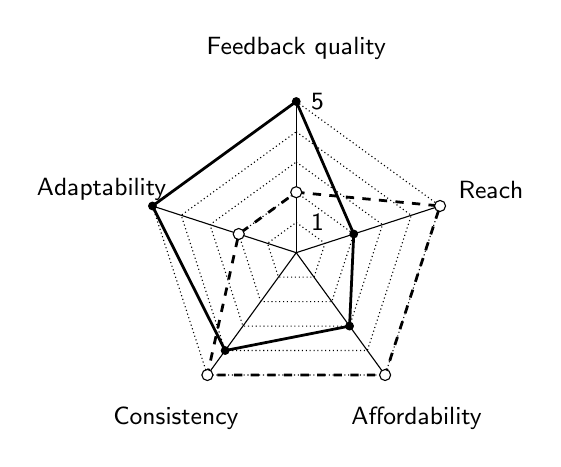
\begin{tikzpicture}[scale=.8,font=\sffamily\small]
\foreach \r in {1,2,3,4,5}{
  \draw[densely dotted] (90:{\r*.48})--(18:{\r*.48})--(-54:{\r*.48})--(-126:{\r*.48})--(162:{\r*.48})--cycle;}
\foreach \a/\label in {90/Feedback quality,18/Reach,-54/Affordability,-126/Consistency,162/Adaptability}{
  \draw (0,0)--(\a:2.4);\node[align=center] at (\a:3.25){\label};}
\draw[line width=1pt] (90:2.4)--(18:.96)--(-54:1.44)--(-126:1.92)--(162:2.4)--cycle;
\draw[line width=1pt,dashed] (90:.96)--(18:2.4)--(-54:2.4)--(-126:2.4)--(162:.96)--cycle;
\foreach \a/\r in {90/2.4,18/.96,-54/1.44,-126/1.92,162/2.4}{\fill (\a:\r) circle(2pt);}
\foreach \a/\r in {90/.96,18/2.4,-54/2.4,-126/2.4,162/.96}{\draw[fill=white] (\a:\r) circle(2.5pt);}
\node[anchor=west] at (.08,.48) {1};\node[anchor=west] at (.08,2.4) {5};
\end{tikzpicture}
\par\smallskip{\sffamily\small Solid + filled point: live cohort\quad Dashed + open point: self-paced}
\caption{An illustrative delivery profile. Every axis uses the same 1--5
scale and points outwards from weak to strong. The shape is not a score.}
\FigureSource{Hypothetical founder ratings; no survey or empirical comparison is implied.}
\end{figure}

The live cohort looks more adaptable, while the self-paced course looks easier
to distribute. Neither conclusion settles the choice. A founder serving novices
who need frequent correction may accept limited reach. A founder teaching a
stable, well-specified procedure may make a different tradeoff.

Do not compare polygon areas or add these ratings into a total without a
reasoned model of the criteria and their weights. An ordinal rating does not
establish equal distances between categories. If precise comparison matters,
print the underlying values in a table alongside the chart.

\section{Follow the money through the promise}
The economics can be read as a sequence too. Begin with revenue, subtract each
direct cost once, and ask what remains to pay for the wider enterprise. A
waterfall makes that sequence visible. Its floating bars show changes; the
first and final bars show totals.

\begin{figure}[H]
\centering
\begin{tikzpicture}[x=1.1cm,y=.014cm,font=\sffamily\scriptsize]
\draw[->] (-.6,0)--(7.5,0);
\draw[->] (-.6,0)--(-.6,275);
\foreach \n in {0,60,120,180,240}{\draw (-.7,\n)--(-.6,\n);\node[anchor=east] at(-.8,\n){\n};}
\node[anchor=west] at(-.5,274){INR thousands};
\filldraw[fill=white,pattern=north east lines] (0,0) rectangle(.65,240);
\filldraw[fill=white] (1.5,195) rectangle(2.15,240);
\filldraw[fill=white] (3,165) rectangle(3.65,195);
\filldraw[fill=white] (4.5,150) rectangle(5.15,165);
\filldraw[fill=white,pattern=north east lines] (6,0) rectangle(6.65,150);
\draw[dashed] (.65,240)--(1.5,240) (2.15,195)--(3,195) (3.65,165)--(4.5,165) (5.15,150)--(6,150);
\foreach \x/\y/\label in {.325/250/240,1.825/250/{-45},3.325/205/{-30},4.825/175/{-15},6.325/160/150}{\node at(\x,\y){\label};}
\foreach \x/\label in {.325/Revenue,1.825/Teaching,3.325/Feedback,4.825/Materials,6.325/Contribution}{\node[anchor=north,align=center] at(\x,-8){\label};}
\end{tikzpicture}
\caption{From revenue to contribution in an illustrative twenty-person cohort.
Negative labels are costs. Contribution is a subtotal before overhead and tax.}
\FigureSource{Synthetic INR amounts consistent with the earlier cohort table.}
\end{figure}

The last bar is not personal income. It must still cover rent, central staff,
marketing, unsuccessful experiments, and tax. Nor does a positive contribution
establish that the business has enough cash today: payments and expenses can
arrive at different times. A useful model makes those boundaries visible.

\begin{DecisionChecklist}{Is this promise ready to scale?}
\item Define the customer's result in a form you can observe.
\item Identify a handoff or failure that could prevent that result.
\item Include support and recovery in the delivery cost.
\item Choose the evidence that would make you pause expansion.
\end{DecisionChecklist}

\LessonTakeaway{Design the promised change and the system that pays for it
together. A useful outcome without a viable delivery model is hard to sustain;
a profitable delivery model without a useful outcome is hard to defend.}

\CaseStudies{Three fictional founders ask what must happen behind the scenes
for a customer to receive the promised result. Make your choice before reading
the proposed move.}

\CaseStudy{1}{TECHNOLOGY}{A useful answer, every Monday}
  {Aarav\quad /\quad Receivables software\quad /\quad First five customers}
Aarav's assistant lists overdue invoices. Its demonstrations look excellent,
but the accounting manager keeps a spreadsheet open beside it. A failed data
connection and a changed payment-status field have both produced confident,
incorrect answers.

\CaseSection{The decision}
Prospects request forecasts. Current users ask whether they can trust the
invoice list. Should Aarav spend the next fortnight adding a forecasting screen
or making the existing answer reliable?

\CasePrompt{Write the customer's promised result in one sentence. What evidence
would let the manager act without rechecking every record?}

\CaseSection{A defensible move}
Start with the existing promise. Aarav adds a last-sync time, an exception list,
and a rule that withholds an answer when a material source is unavailable. He
agrees an escalation procedure with each customer. For four Mondays, he checks
whether the manager can make the collections decision without rebuilding the
analysis.

The measure is not the number of answers generated. It is the number of
weekly decisions that cross the customer's reliability threshold. Human review
may be necessary initially. Its cost belongs in the delivery model rather than
being hidden as the founder's unpaid time.

\CaseSection{What would change the answer?}
If reliable collection decisions already happen and forecasting is the binding
constraint, the new screen becomes a sensible candidate. The lesson is to find
the failed link in the promise before choosing the feature.

\CaseStudy{2}{FASHION}{The dress that arrives on time}
  {Mira\quad /\quad Small occasionwear label\quad /\quad Pre-order launch}
Mira's customers love the sample photographs. Her first launch sells thirty
pre-orders, each needed for a particular occasion. The workshop can make the
dresses, but the quoted production time excludes fabric inspection, alterations,
and courier delays. Two customers ask whether their orders will arrive before
the weddings they are attending.

\CaseSection{The decision}
A supplier offers a discount if Mira doubles the batch. Larger production could
improve the margin per dress. It would also use nearly all her cash and leave
little room for remakes. Should she take the discount?

\CasePrompt{What is the product from this customer's point of view? Name two
handoffs that could break the promise even if the dress itself is well made.}

\CaseSection{A defensible move}
Mira treats fit and arrival date as parts of the offering. She works backwards
from each customer's occasion, confirms measurements before cutting, inspects
fabric before committing the batch, and reserves time for alterations. She
publishes an order cut-off based on that complete sequence.

Before expanding, she counts orders delivered at the agreed fit and date,
records remake costs, and includes customer-support time in the contribution
calculation. The supplier's unit-price discount matters only if the larger
batch preserves the whole promise and leaves enough cash to recover from
plausible failures.

\CaseSection{What would change the answer?}
A repeat collection with stable sizing, replenishable fabric, and spare workshop
capacity may justify a larger batch. A pre-order deadline tied to an event has
different economics from an everyday item that customers can wait for.

\CaseStudy{3}{EDUCATION}{Beyond finishing the course}
  {Leela\quad /\quad Practical analytics course\quad /\quad First paid cohort}
Leela teaches professionals to diagnose operational problems with data. Her
learners enjoy the sessions and most finish the course. Yet several cannot
choose an appropriate method when the problem differs from the worked example.
The satisfaction survey is positive. The promised capability remains uncertain.

\CaseSection{The decision}
Leela wants to enrol sixty learners next time instead of twenty. She can record
more lectures or invest the same time in designing better practice and feedback.
What must she know before deciding?

\CasePrompt{Design one unfamiliar assessment task. What would count as an
independent diagnosis, and how would you apply that standard consistently?}

\CaseSection{A defensible move}
First define the result. Leela asks learners to inspect an unfamiliar dataset,
state the operational question, defend a method, and explain one limitation.
She uses the same rubric before and after the course and keeps completion and
independent performance as separate measures.

She then examines the failed attempts. If learners can follow procedures but
cannot select among them, another lecture may add little. Contrasting problems,
worked reasoning, and feedback on the choice of method could address the actual
gap. She tests that change in a small group before scaling the full course.

\CaseSection{What would change the answer?}
If the learning mechanism works but access is the main obstacle, recording
sessions may be valuable. The right format follows the learner's constraint.
It does not follow automatically from the founder's wish to increase enrolment.

\clearpage
\section*{Compare the decisions}
Aarav needs a trustworthy answer, Mira needs a dependable arrival, and Leela
needs independent capability. The sectors differ; the reasoning travels.
Define the change, trace the mechanism, test the weak link, and include the
cost of reliability in the model.

\begin{table}[H]
\centering\small\sffamily
\begin{tabularx}{\linewidth}{@{}p{.72in}>{\raggedright\arraybackslash}X>{\raggedright\arraybackslash}X@{}}
\toprule
\textbf{Founder} & \textbf{Evidence of the promise} & \textbf{Hidden delivery work}\\
\midrule
Aarav & A decision without rebuilding the analysis & Data checks and exception handling\\
Mira & The agreed fit by the agreed date & Inspection, alterations, recovery time\\
Leela & Independent diagnosis on an unfamiliar task & Practice design, assessment, feedback\\
\bottomrule
\end{tabularx}
\caption{The same lesson under three different sets of constraints. The cases
illustrate reasoning; they are not documented company histories.}
\end{table}

\begin{LessonReview}
\item Specify the change the customer needs, rather than a list of features.
\item Test the work that makes that change reliable, including recovery from failure.
\item Treat contribution as a subtotal with explicit cost boundaries.
\end{LessonReview}
\TransferQuestion{Which part of your promise currently depends on unrecorded work by the founder, and what would happen if demand doubled?}

\NotesSection
The opening reading excerpts come from the existing Chapter 1, ``Why Play the
Game?'', and Chapter 10, ``The Theory of Product and Service Design.'' They are
included to evaluate sustained reading in the new format. The charts, cohort
arithmetic, and three founder cases were written for this design specimen.
Every dataset and founder in those examples is illustrative. Production
chapters should replace these with their own evidence, notes, and finished cases.
\end{document}
